\chapter{Design}

\section{Architecture}

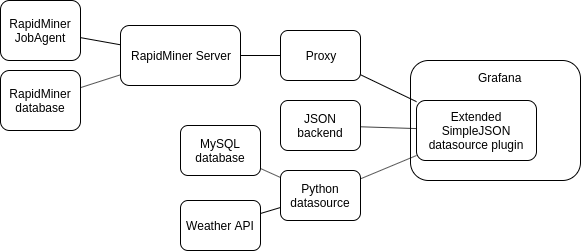
\includegraphics{figures/architecture.png}

\begin{itemize}
	\item why do we need a gateway
	\item how can we access data from RapidMiner WebService
	\item why is it good to have a python compoment between Grafana and MySQL
	\begin{itemize}
		\item we can customize it better, what we see from the database
		\item can implement business logic, only see business-relevant projections, granularity of the data
		\item can aggregate data from different backends
		\item can aggregate data with outsider APIs (POC implementation for this use-case)
	\end{itemize}
\end{itemize}

\section{Components}

\begin{itemize}
	\item Responsibilities
	\item Interfaces?
\end{itemize}

\begin{itemize}
	\item Grafana
	\item proxy/gateway
	\item python-datasource
	\begin{itemize}
		\item python-datasource
		\item mysql
		\item weather-api
	\end{itemize}
	\item RapidMiner stack
	\begin{itemize}
		\item rapidminer-server
		\item job-agent
		\item database
	\end{itemize}
	\item Grafana datasource plugin (extended API - parameters)
	\begin{itemize}
		\item extended API for asking for available parameters
		\item extended GUI, that dynamically lists available parameters
	\end{itemize}
	\item Grafana extended panel plugin
\end{itemize}